A basic obstruction-free queue is given in Listing \ref{lst:queue}. From this
queue, the authors construct a wait-free queue by using the fast-path-slow-path
methodology. This queue is similar to the base used in the LCRQ algorithm.

$FAA(x, v)$ atomically reads the value stored in the $x$ variable, and
increments it by $v$. $CAS(x, t, v)$ atomically reads the value stored in $x$,
compares it to $t$ and, if $x$ is equal to $t$ (success), replaces the value of
$x$ by $v$. $CAS$ returns whether it has successfully replaced the value or not.

\begin{lstlisting}[mathescape,
                   frame=single,
                   caption={An obstruction-free queue using an infinite array.},
                   label={lst:queue},
                   language=C]
Q: queue
T: pointer to tail
H: pointer to head
enqueue(x: var) {
  do t := FAA(&T, 1);
  while (!CAS(&Q[t], $\bot$, x));
}
dequeue(x: var) {
  do h := FAA(&H, 1);
  while (!CAS(&Q[h], $\bot$, $\top$) and T > h);
  return (Q[h] == T ? EMPTY : Q[h]);
}
\end{lstlisting}

\para{Basic queue} This queue uses a shared (emulated) infinite array to
store elements. We will see later how this is done and how memory can be
reclaimed. Two special values are reserved : $\bot$ (bottom) and $\top$ (top).
$\bot$ stands for empty cells as the queue is initially filled with $\bot$.
$\top$ stands for unusable cells. When one thread dequeues an element, it marks
the cells with $\top$ to prevent other threads to enqueue an element in it.

To enqueue an element, one thread tries to find an available cell on the array,
a cell marked with $\bot$. One cannot enqueue an element in a $\top$ marked cell
because it could violate the FIFO property of the queue. To get a unique index
on the array, one thread uses fetch-and-add to increment the shared tail
reference. Considering the reference is shared by all threads, using
compare-and-swap instead of fetch-and-add would result in lots of failures.
After one thread is given a unique index, it needs to certify that the cell is
empty. He then uses compared-and-swap to enqueue an element into the array. In
the event of compare-and-swap failure, the thread redoes the whole process until
the element is enqueued.

The dequeue operation works in a similar manner, one thread tries to find either a
cell filled with an element or marked with $\top$ by using fetch-and-add on a
shared head reference. If a thread stops on a $\top$ marked cell, the dequeue
returns \texttt{EMPTY}.

This queue is designed to be fast. Dequeue may always fail if queued values are
dequeued by another thread. Enqueue may always fail if another thread marks each
empty cell unusable. As a result, it is neither wait-free or lock-free because
it is prone to livelocking. As only one thread is guaranteed to progress, this
queue is only obstruction-free. \\

\begin{figure}
    \caption{The fast-path-slow-path methodology \cite{Kogan:2012:MCF:2370036.2145835}.}
    \label{fig:fpsp}
    \center
    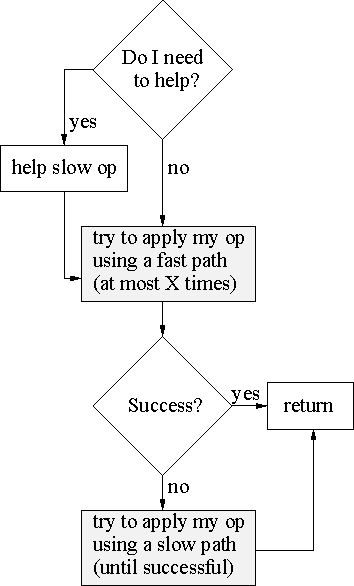
\includegraphics[width=0.6\linewidth]{img/fpsp.pdf}
\end{figure}

\para{Fast-path-slow-path} To construct a wait-free realization of the previous
queue, the authors use the fast-path-slow-path methodology. As shown in figure
\ref{fig:fpsp}, one thread tries to enqueue or dequeue an element using a
fast-path, which is similar to the previous queue. A maximum number of failures
is set. If a thread failed too many times to apply its operation, it falls back
on a slow-path.

For example, if a thread fails to enqueue an element, it publishes an enqueue
request. When other threads want to dequeue an element, they look at all pending
enqueue requests, and eventually help one request to complete. The enqueuer
thread then keeps trying to enqueue the element until it or another succeeds.

Threads are linked in a ring, they keep a reference to a \textit{peer} to which
they help the operation to complete. Each time a thread successfully helps
another thread, it updates his \textit{peer} to the next thread in the ring so
that each
thread happens to help every one at some point. \\

\para{Memory reclamation} The authors designed their queue with an infinite
array. To do so, the queue is split into segments as a linked list. Each segment
contains a fixed number of cells. The list of segments is expanded as necessary.
Because the tail and head pointers are never decremented, segments no longer in
use need to be freed.

After one thread dequeues an element, the thread tries to reclaim memory from
unused segments. They use compare-and-swap to achieve mutual exclusion so that
if several threads try to reclaim memory, only one should succeed. Unused
segments are segments filled with $\top$ marked cells. Each thread keeps a
reference to its currently used segment. The \textit{cleaner} thread ensures
that no thread keeps a reference to a segment about to be freed and changes it
if needed. \\

\para{Wait-free guaranty} The number of tries on the lock-free fast-past is
bounded. After sufficient failures, the algorithm falls back on the slow-path.
Each thread helps every other thread at some point. If the operation of one
thread continuously fails to complete, it will definitely complete when all
other threads become his helper.
